\section{Рабочий проект}
\subsection{Спецификация компонентов и классов программы}

\subsection{Модуль shift.py}

Модуль shift.py содержит функцию для случайного сдвига изображения по осям X и Y. Модуль не содержит классов. Метод модуля - shift image. Он выполняет случайный сдвиг изображения на расстояние, не превышающее заданный процент от его размеров, с использованием аффинного преобразования. Входные данные:

\begin{itemize}
	\item image (тип PIL.Image.Image) – исходное изображение для сдвига;
	\item max shift (тип float, значение по умолчанию = 0.1) – максимальный процент сдвига от размера изображения.
\end{itemize}

Возвращаемые данные: PIL.Image.Image – изображение после сдвига.

\subsection{Модуль brightness.py}

Модуль brightness.py предоставляет функцию для изменения яркости изображения. Модуль не содержит классов. Метод модуля - change brightness. Он изменяет яркость изображения с использованием класса ImageEnhance.Brightness из библиотеки Pillow. Входные данные:

\begin{itemize}
	\item image (тип PIL.Image.Image) – исходное изображение;
	\item factor (тип float, значение по умолчанию = 1.0) – коэффициент яркости (меньше 1 – затемнение, больше 1 – осветление).
\end{itemize}

Возвращаемые данные: PIL.Image.Image – изображение с измененной яркостью.

\subsection{Модуль rotate.py}

Модуль rotate.py содержит функцию для поворота изображения на заданный угол. Модуль не содержит классов. Метод модуля - rotate image. Он выполняет поворот изображения на заданный угол с возможностью изменения размера после поворота. Входные данные:

\begin{itemize}
	\item image (тип PIL.Image.Image) – исходное изображение;
	\item angle (тип float) – угол поворота в градусах;
	\item target size (тип tuple, необязательный) – целевой размер изображения после поворота (ширина, высота).
\end{itemize}

Возвращаемые данные: PIL.Image.Image – повернутое изображение (и измененного размера, если указан target size).

\subsection{Модуль flip.py}

Модуль flip.py предоставляет функцию для отражения изображения по горизонтали или вертикали. Модуль не содержит классов. Метод модуля - flip image. Он отражает изображение по горизонтали или вертикали с использованием метода transpose из библиотеки Pillow. При некорректном значении параметра mode вызывает исключение ValueError. Входные данные:

\begin{itemize}
	\item image (тип PIL.Image.Image) – исходное изображение;
	\item mode (тип str, значение по умолчанию = 'horizontal') – режим отражения (horizontal или vertical).
\end{itemize}

Возвращаемые данные: PIL.Image.Image – отраженное изображение.

\subsection{Модуль noise.py}

Модуль noise.py содержит функцию для добавления шума к изображению в градациях серого. Модуль не содержит классов. Метод модуля - add noise. Он добавляет к изображению шум типа "гауссовский" или "соль и перец". Для обработки используется библиотека NumPy. Требует, чтобы изображение было в режиме L, иначе вызывает исключение ValueError. Входные данные:

\begin{itemize}
	\item image (тип PIL.Image.Image) – исходное изображение в режиме L (градации серого);
	\item noise type (тип str, значение по умолчанию = 'gaussian') – тип шума (gaussian или salt pepper);
	\item **kwargs – дополнительные параметры:
	\begin{itemize}
		\item для gaussian: stddev (тип float, значение по умолчанию = 10) – стандартное отклонение шума;
		\item для salt pepper: amount (тип float, значение по умолчанию = 0.05) – доля пикселей, затронутых шумом; salt vs pepper (тип float, значение по умолчанию = 0.5) – соотношение "соли" и "перца".
	\end{itemize}
\end{itemize}

Возвращаемые данные: PIL.Image.Image – изображение с добавленным шумом.

\subsection{Модуль augmentation config.py}

Модуль augmentation config.py определяет конфигурацию аугментаций. Модуль не содержит классов или методов, представляя собой словарь augmentation config. Описание конфигурации:

\begin{itemize}
	\item available augmentations (тип list) – список доступных аугментаций: noise, rotate, flip, shift, brightness;
	\item noise, rotate, flip, shift, brightness (тип dict) – настройки для каждой аугментации с полями enabled и params (например, angle range, std range);
	\item volume presets (тип dict) – предустановленные объемы генерации: 1х25, 1х50, 1х100.
\end{itemize}

Он обеспечивает централизованное управление параметрами аугментаций и их состоянием.

\subsection{Модуль pipeline.py}

Модуль pipeline.py реализует логику применения аугментаций. Он обеспечивает централизованное управление параметрами аугментаций и их состоянием. Методы модуля представлены в таблице ~\ref{table:pipeline}.

\renewcommand{\arraystretch}{0.8} % уменьшение расстояний до сетки таблицы
\begin{xltabular}{\textwidth}{|>{\hsize=0.9\hsize\raggedright\arraybackslash}X|
		>{\hsize=1.0\hsize\setlength{\baselineskip}{0.7\baselineskip}}X|
		>{\hsize=1.0\hsize}X|
		>{\hsize=1.3\hsize}X|}
	\caption{Методы модуля pipeline.py\label{table:pipeline}}\\
	\hline 
	\centrow \setlength{\baselineskip}{0.7\baselineskip} Название метода & 
	\centrow Параметры метода &
	\centrow Возвращаемое значение & 
	\centrow Назначение метода \\ 
	\hline 
	\endfirsthead
	
	\caption*{Продолжение таблицы \ref{table:pipeline}}\\
	\hline 
	\centrow Название метода & 
	\centrow Параметры метода &
	\centrow Возвращаемое значение & 
	\centrow Назначение метода \\ 
	\hline 
	\endhead
	
	\_\_init\_\_ & Не имеет & Не имеет  & Инициализирует главное окно программы, задает его параметры, заголовок, панель меню с действиями для переключения режимов \\ \hline 
	
	apply\_ augmentation & image (тип PIL.Image. Image) – изображение; augmentation\_ type (тип str) – тип аугментации & PIL.Image. Image – аугментированное изображение & Применяет одну аугментацию в соответствии с конфигурацией.\\
	\hline
	
	process\_ images & image (тип PIL.Image. Image) – изображение; target\_size (тип tuple) – размер; volume\_level (тип str, по умолчанию 'low') – уровень генерации & list – список аугментированных изображений & Генерирует заданное количество аугментированных версий с случайными комбинациями аугментаций.\\
	\hline
	
	process\_ images & image (тип PIL.Image. Image) – изображение; target\_size (тип tuple) – размер; volume\_level (тип str, по умолчанию 'low') – уровень генерации & list – список аугментированных изображений & Генерирует заданное количество аугментированных версий с случайными комбинациями аугментаций.\\
	\hline
	
\end{xltabular}
\renewcommand{\arraystretch}{1.0} % восстановление сетки
\vspace{-\baselineskip}


\subsection{Модуль main\_window.py}

Модуль main\_window предоставляет графический интерфейс для взаимодействия с пользователем, включая загрузку изображений, выбор директории, настройку аугментаций, предпросмотр и сохранение результатов. Константы и методы: отсутствуют.

Класс MainWindow (модуль main\_window.py)

Базовый класс: AugmentationWindow (из модуля ui.window).

Внутренние поля представлены в таблице ~\ref{table:main_window}

\begin{xltabular}{\textwidth}{|X|X|X|}
	\caption{Внутренние поля класса MainWindow \label{table:main_window}} \\
	\hline 
	\centrow Внутреннее поле & 
	\centrow Тип & 
	\centrow Описание \\ 
	\hline 
	\endfirsthead
	
	\caption*{Продолжение таблицы \ref{table:main_window}} \\
	\hline 
	\centrow Внутреннее поле & 
	\centrow Тип & 
	\centrow Описание \\ 
	\hline 
	\endhead
	
	output\_dir & str или None & Путь к директории для сохранения результатов. \\ \hline
	image\_paths & list & Список путей к загруженным изображениям. \\ \hline
	progress\_bar & QProgressBar & Виджет для отображения прогресса обработки. \\ \hline
	scroll\_area & QScrollArea & Область прокрутки для отображения миниатюр. \\ \hline
	preview\_container & QWidget & Контейнер для размещения миниатюр аугментированных изображений. \\ \hline
	preview\_layout & QHBoxLayout & Макет для размещения миниатюр. \\ \hline
	select\_augs\_button & QPushButton & Кнопка для открытия диалога выбора аугментаций. \\ \hline
\end{xltabular}

Методы класса представлены в таблице ~\ref{table:main_window_method}

\renewcommand{\arraystretch}{0.8} % уменьшение расстояний до сетки таблицы
\begin{xltabular}{\textwidth}{|>{\hsize=0.9\hsize\raggedright\arraybackslash}X|
		>{\hsize=1.0\hsize\setlength{\baselineskip}{0.7\baselineskip}}X|
		>{\hsize=1.0\hsize}X|
		>{\hsize=1.3\hsize}X|}
	\caption{Методы модуля pipeline.py\label{table:main_window_method}}\\
	\hline 
	\centrow \setlength{\baselineskip}{0.7\baselineskip} Название метода & 
	\centrow Параметры метода &
	\centrow Возвращаемое значение & 
	\centrow Назначение метода \\ 
	\hline 
	\endfirsthead
	
	\caption*{Продолжение таблицы \ref{table:main_window_method}}\\
	\hline 
	\centrow Название метода & 
	\centrow Параметры метода &
	\centrow Возвращаемое значение & 
	\centrow Назначение метода \\ 
	\hline 
	\endhead
	
	load\_images & Не имеет & Не имеет  & Загружает изображения из выбранной папки и отображает предпросмотр первого. \\ \hline
	
	select\_output \_folder & Не имеет & Не имеет  & Загружает изображения из выбранной папки и отображает предпросмотр первого. \\ \hline

	open\_output\_ directory & Не имеет & Не имеет  & Открывает папку с результатами в файловом менеджере. \\ \hline 

	show\_image \_preview & path (тип str) – путь к изображению & Не имеет  & Отображает предпросмотр исходного изображения в интерфейсе. \\ \hline 

	show\_ augmented\_ preview & pil\_image (тип PIL.Image.Image) – аугментированное изображение & Не имеет & Отображает предпросмотр аугментированного изображения в интерфейсе. \\ \hline
	
	apply\_ selected\_ augmentation & Не имеет & Не имеет & Выполняет аугментацию для всех загруженных изображений и сохраняет результаты. \\ \hline
	
	open\_ augmentation \_selector & Не имеет & Не имеет & Открывает диалог для настройки активных аугментаций. \\ \hline
	
	apply\_ augmentation & image (тип PIL.Image. Image) – изображение; augmentation\_ type (тип str) – тип аугментации & PIL.Image. Image – аугментированное изображение & Применяет одну аугментацию в соответствии с конфигурацией.\\
	\hline
	
	process\_ images & image (тип PIL.Image. Image) – изображение; target\_size (тип tuple) – размер; volume\_level (тип str, по умолчанию 'low') – уровень генерации & list – список аугментированных изображений & Генерирует заданное количество аугментированных версий с случайными комбинациями аугментаций.\\
	\hline
	
	process\_ images & image (тип PIL.Image. Image) – изображение; target\_size (тип tuple) – размер; volume\_level (тип str, по умолчанию 'low') – уровень генерации & list – список аугментированных изображений & Генерирует заданное количество аугментированных версий с случайными комбинациями аугментаций.\\
	\hline
	
\end{xltabular}
\renewcommand{\arraystretch}{1.0} % восстановление сетки
\vspace{-\baselineskip}

\subsection{Модуль augmentation\_selector.py}

Модуль augmentation\_selector.py предоставляет диалоговое окно для выбора активных аугментаций. Константы: отсутствуют. Метод get\_selected\_augmentations возвращает список аугментаций, отмеченных пользователем.

Внутренние поля представлены в таблице ~\ref{table:table:augmentation_selector}

\begin{xltabular}{\textwidth}{|X|X|X|}
	\caption{Внутренние поля класса MainWindow \label{table:augmentation_selector}} \\
	\hline 
	\centrow Внутреннее поле & 
	\centrow Тип & 
	\centrow Описание \\ 
	\hline 
	\endfirsthead
	
	\caption*{Продолжение таблицы \ref{table:main_window}} \\
	\hline 
	\centrow Внутреннее поле & 
	\centrow Тип & 
	\centrow Описание \\ 
	\hline 
	\endhead
	
	selected & set & Множество выбранных пользователем аугментаций. \\ \hline
	checkboxes & dict & Словарь, где ключ – название аугментации, значение – QCheckBox. \\ \hline
\end{xltabular}

\subsection{Модульное тестирование разработанной программной системы}

Модульное тестирование проведено для проверки корректности работы отдельных компонентов программной системы аугментации изображений. Тестирование осуществлялось путем создания простых тестовых скриптов на языке Python без использования сторонних библиотек тестирования. Для каждого теста указаны назначение, код и результат, полученный при его выполнении. Тесты выполнялись на тестовом изображении размером 100x100 пикселей, созданном программно с использованием библиотеки Pillow, а результаты проверялись визуально (путем анализа сохраненных файлов) и программно (сравнением параметров).


Тест 1: Проверка функции сдвига изображения (shift.py)
Назначение теста: Проверить, что функция shift\_image корректно выполняет случайный сдвиг изображения в пределах заданного диапазона.

\begin{figure}[H]
	\begin{lstlisting}[language=Python]
		from PIL import Image
		from augmentor import shift_image
		
		test_image = Image.new('RGB', (100, 100), color='white')
		test_image.save('test_original_shift.png')
		
		
		
		shifted_image = shift_image(test_image, max_shift=0.2)
		shifted_image.save('test_shifted.png')
		
		
		if shifted_image.size == test_image.size:
		print("Тест пройден: размеры изображения сохранены после сдвига.")
		else:
		print("Тест провален: размеры изображения изменились после сдвига.")
	\end{lstlisting}  
	\caption{Модульный тест функции shift\_image}
	\label{model_test:test1}
\end{figure}

Результат тестирования:
\begin{figure}[H]
	\centering
	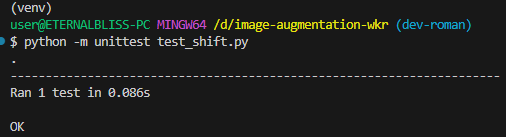
\includegraphics[width=0.7\linewidth]{images/resulttest1}
	\caption{Результат тестирования функции shift\_image}
	\label{fig:resulttest1}
\end{figure}

Тест 2: Проверка функции изменения яркости (brightness.py)
Назначение теста: Убедиться, что функция change\_brightness корректно изменяет яркость изображения в зависимости от заданного коэффициента.

\begin{figure}[H]
	\begin{lstlisting}[language=Python]
		from PIL import Image
		import numpy as np
		from augmentor import change_brightness
		
		test_image = Image.new('RGB', (100, 100), color=(128, 128, 128))
		test_image.save('test_original_brightness.png')
		
		
		bright_image = change_brightness(test_image, factor=1.5)
		bright_image.save('test_brightened.png')
		
		
		bright_array = np.array(bright_image)
		original_array = np.array(test_image)
		if bright_array.mean() > original_array.mean():
		print("Тест пройден: яркость изображения увеличилась.")
		else:
		print("Тест провален: яркость не изменилась или уменьшилась.")



	\end{lstlisting}  
	\caption{Модульный тест функции change\_brightness}
	\label{model_test:test2}
\end{figure}

Результат тестирования:
\begin{figure}[H]
	\centering
	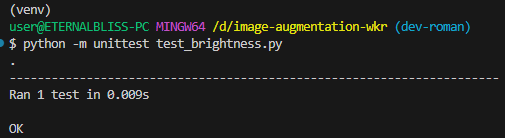
\includegraphics[width=0.7\linewidth]{images/resulttest2}
	\caption{Результат тестирования функции change\_brightness}
	\label{fig:resulttest2}
\end{figure}

Тест 3: Проверка функции поворота изображения (rotate.py)
Назначение теста: Проверить, что функция rotate\_image корректно поворачивает изображение на заданный угол.

\begin{figure}[H]
	\begin{lstlisting}[language=Python]
		from PIL import Image
		from augmentor import rotate_image
		
		test_image = Image.new('RGB', (100, 100), color='white')
		test_image.save('test_original_rotate.png')
		
		
		rotated_image = rotate_image(test_image, angle=90, target_size=(100, 100))
		rotated_image.save('test_rotated.png')
		
		if rotated_image.size == (100, 100):
		print("Тест пройден: изображение повернуто и размер скорректирован.")
		else:
		print("Тест провален: размер изображения не соответствует ожидаемому.")
	\end{lstlisting}  
	\caption{Модульный тест функции rotate\_image}
	\label{model_test:test3}
\end{figure}

Результат тестирования:
\begin{figure}[H]
	\centering
	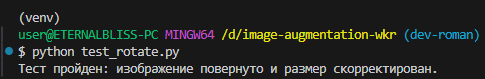
\includegraphics[width=0.7\linewidth]{images/resulttest3}
	\caption{Результат тестирования функции rotate\_image}
	\label{fig:resulttest3}
\end{figure}

Тест 4: Проверка функции отражения изображения (flip.py)
Назначение теста: Убедиться, что функция flip\_image корректно отражает изображение по вертикали.

\begin{figure}[H]
	\begin{lstlisting}[language=Python]
		from PIL import Image
		from augmentor import flip_image
		
		test_image = Image.new('RGB', (100, 100), color='black')
		test_image.save('test_original_flip.png')
		
		flipped_image = flip_image(test_image, mode='vertical')
		flipped_image.save('test_flipped.png')
		
		try:
		flipped_image.save('test_flipped.png')
		print("Тест пройден: изображение отражено по вертикали.")
		except Exception as e:
		print(f"Тест провален: ошибка при отражении - {e}")
	\end{lstlisting}  
	\caption{Модульный тест функции flip\_image}
	\label{model_test:test4}
\end{figure}

Результат тестирования:
\begin{figure}[H]
	\centering
	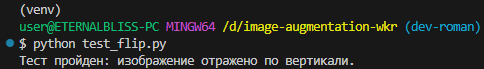
\includegraphics[width=0.7\linewidth]{images/resulttest4}
	\caption{Результат тестирования функции flip\_image}
	\label{fig:resulttest4}
\end{figure}

Тест 5: Проверка функции добавления шума (noise.py)
Назначение теста: Проверить, что функция add\_noise корректно добавляет гауссовский шум к изображению в градациях серого.

\begin{figure}[H]
	\begin{lstlisting}[language=Python]
		from PIL import Image
		import numpy as np
		from augmentor import add_noise
		
		test_image = Image.new('L', (100, 100), color=128)
		test_image.save('test_original_noise.png')
		
		noisy_image = add_noise(test_image, noise_type='gaussian', stddev=15)
		noisy_image.save('test_noisy.png')
		
		original_array = np.array(test_image)
		noisy_array = np.array(noisy_image)
		if noisy_array.var() > original_array.var():
		print("Тест пройден: шум добавлен, дисперсия увеличилась.")
		else:
		print("Тест провален: дисперсия не изменилась.")
	\end{lstlisting}  
	\caption{Модульный тест функции add\_noise}
	\label{model_test:test5}
\end{figure}

Результат тестирования:
\begin{figure}[H]
	\centering
	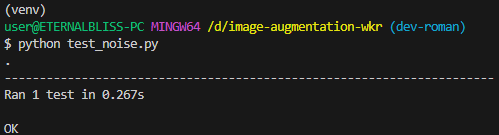
\includegraphics[width=0.7\linewidth]{images/resulttest5}
	\caption{Результат тестирования функции add\_noise}
	\label{fig:resulttest5}
\end{figure}

Тест 6: Проверка функции генерации аугментированных изображений (pipeline.py)
Назначение теста: Проверить, что функция process\_images корректно генерирует заданное количество аугментированных изображений.

\begin{figure}[H]
	\begin{lstlisting}[language=Python]
		from PIL import Image
		import os
		from core.pipeline import process_images
		from config.augmentation_config import augmentation_config
		
		test_image = Image.new('RGB', (100, 100), color='white')
		test_image.save('test_original_pipeline.png')
		
		augmentation_config['volume_presets']['1х25'] = 3
		results = process_images(test_image, target_size=(100, 100), volume_level='1х25')
		
		for i, img in enumerate(results):
		img.save(f'test_pipeline_aug_{i}.png')
		
		if len(results) == 3:
		print("Тест пройден: сгенерировано 3 аугментированных изображения.")
		else:
		print("Тест провален: количество изображений не соответствует ожидаемому.")
	\end{lstlisting}  
	\caption{Модульный тест функции process\_images}
	\label{model_test:test6}
\end{figure}

Результат тестирования:
\begin{figure}[H]
	\centering
	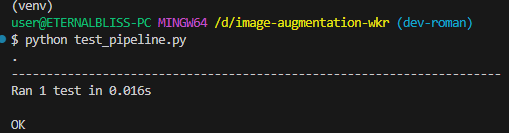
\includegraphics[width=0.7\linewidth]{images/resulttest6}
	\caption{Результат тестирования функции process\_images}
	\label{fig:resulttest6}
\end{figure}

Тест 7: Проверка загрузки изображений и интерфейса (main\_window.py)
Назначение теста: Проверить, что класс MainWindow корректно загружает изображения и отображает их в интерфейсе.

\begin{figure}[H]
	\begin{lstlisting}[language=Python]
		from PIL import Image
		import os
		from ui.main_window import MainWindow
		from PySide6.QtWidgets import QApplication
		
		app = QApplication([])
		
		os.makedirs('test_folder', exist_ok=True)
		test_image = Image.new('RGB', (100, 100), color='white')
		test_image.save('test_folder/test_image.png')
		
		main_window = MainWindow()
		main_window.image_paths = ['test_folder/test_image.png']
		main_window.load_images()
		
		if main_window.image_count == 1:
		print("Тест пройден: одно изображение успешно загружено.")
		else:
		print("Тест провален: изображение не загружено.")
	\end{lstlisting}  
	\caption{Модульный тест класса MainWindow}
	\label{model_test:test7}
\end{figure}

Результат тестирования:
\begin{figure}[H]
	\centering
	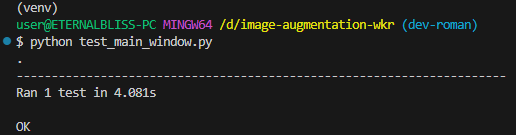
\includegraphics[width=0.7\linewidth]{images/resulttest7}
	\caption{Результат тестирования класса MainWindow}
	\label{fig:resulttest7}
\end{figure}

Тест 8: Проверка выбора аугментаций в диалоге (augmentation\_selector.py)
Назначение теста: Проверить, что класс AugmentationSelectorDialog корректно сохраняет выбранные пользователем аугментации.

\begin{figure}[H]
	\begin{lstlisting}[language=Python]
		from ui.augmentation_selector import AugmentationSelectorDialog
		from config.augmentation_config import augmentation_config
		from PySide6.QtWidgets import QApplication
		
		app = QApplication([])
		
		available = augmentation_config['available_augmentations']
		selected = ['shift', 'brightness']
		
		dialog = AugmentationSelectorDialog(available, selected)
		
		dialog.checkboxes['rotate'].setChecked(True)
		dialog.checkboxes['shift'].setChecked(True)
		
		selected_augs = dialog.get_selected_augmentations()
		
		if 'rotate' in selected_augs and 'shift' in selected_augs:
		print("Тест пройден: аугментации корректно выбраны.")
		else:
		print("Тест провален: аугментации не соответствуют выбору.")
	\end{lstlisting}  
	\caption{Модульный тест класса AugmentationSelectorDialog}
	\label{model_test:test8}
\end{figure}

Результат тестирования:
\begin{figure}[H]
	\centering
	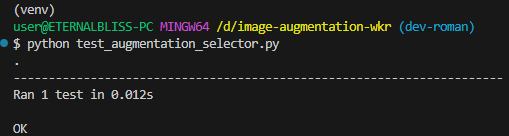
\includegraphics[width=0.7\linewidth]{images/resulttest8}
	\caption{Результат тестирования класса AugmentationSelectorDialog}
	\label{fig:resulttest8}
\end{figure}

\subsection{Системное тестирование разработанной программной системы}

Для проведения системного тестирования были использованы 5 полутоновых изображений 500x500 пикселей в формате jpg. Аугментация проводилась в масштабе - "1к50".

На рисунке~\ref{fig:systest1} представлено главное окно приложения при запуске.
\begin{figure}[H]
	\centering
	\includegraphics[width=0.3\linewidth]{"images/systest1"}
	\caption{Окно приложения при запуске>}
	\label{fig:systest1}
\end{figure}

На рисунке~\ref{fig:systest2} представлено диалоговое окно выбора папки с иходными изображеними.

\begin{figure}[H]
	\centering
	\includegraphics[width=0.5\linewidth]{"images/systest2"}
	\caption{Диалоговое окно выбора выбора папки с иходными изображеними}
	\label{fig:systest2}
\end{figure}

На рисунке~\ref{fig:systest3} представлено диалоговое окно выбора папки, в которой будут генерироваться аугментированные изображения.
\begin{figure}[H]
	\centering
	\includegraphics[width=0.5\linewidth]{"images/systest3"}
	\caption{Диалоговое окно выбора папки, в которой будут генерироваться аугментированные изображения}
	\label{fig:systest3}
\end{figure}

На рисунке~\ref{fig:systest4} представлено диалоговое окно выбора .
\begin{figure}[H]
	\centering
	\includegraphics[width=0.3\linewidth]{"images/systest4"}
	\caption{Результат распознавания нефтяных пятен}
	\label{fig:systest4}
\end{figure}

На рисунке~\ref{fig:systest5} представлено отображение выбора масштаба аугментации.
\begin{figure}[H]
	\centering
	\includegraphics[width=0.3\linewidth]{"images/systest5"}
	\caption{Отображение выбора масштаба аугментации}
	\label{fig:systest5}
\end{figure}

На рисунке~\ref{fig:systest6} представлено отображение выбора методов аугментации.
\begin{figure}[H]
	\centering
	\includegraphics[width=0.3\linewidth]{"images/systest6"}
	\caption{Отображение выбора методов аугментации}
	\label{fig:systest6}
\end{figure}

На рисунке~\ref{fig:systest7} представлено главное окно приложения при запуске.
\begin{figure}[H]
	\centering
	\includegraphics[width=0.5\linewidth]{"images/systest7"}
	\caption{Результат распознавания нефтяных пятен}
	\label{fig:systest7}
\end{figure}
